\documentclass[french]{report}
\usepackage[utf8]{inputenc}
\usepackage[T1]{fontenc}
\usepackage{babel}
\usepackage{fancyhdr}
\usepackage{graphicx}
\usepackage{color}
\usepackage{float}
\usepackage[a4paper,left=1cm,right=1cm,top=1.8cm,bottom=1.8cm]{geometry}
\pagestyle{fancy}
\fancyhf{}
\fancyhead[LE,RO]{Étude conceptuelle}
\fancyhead[RE,LO]{Chapitre 2}
\fancyfoot[CE,CO]{\leftmark}
\fancyfoot[LE,RO]{\thepage}
\setlength{\parindent}{4em}
\setlength{\parskip}{1em}
\renewcommand{\baselinestretch}{1.5}

\begin{document}
\baselineskip=2.0pt
\setcounter{chapter}{1}

\begin{titlepage}
\renewcommand*{\thepage}{\arabic{page}}%
\setcounter{page}{27}%
\newpage
\chapter{
\textit{ Étude conceptuelle }
}
\end{titlepage}
\renewcommand*{\thepage}{\arabic{page}}%
\setcounter{page}{28}%
\newpage
\section{\huge Introduction}     
\LARGE Dans ce chapitre, nous présentons les différentes fonctionnalités que nous voulons voir figurer dans notre projet et détaillons si nécessaire, ainsi que la conception et modélisation de notre application avec ses différents parties.\\
\section{\huge La Conception de notre application :}
\LARGE Développer un système qui transmet et reçoit les données d'un utilisateur en temps réel soulève de nombreux problèmes et difficultés, dans cette étape nous avons voulu essayer d'éliminer ces problèmes et surmonter les difficultés pour nous assurer que notre application aura de bonnes performances.
Pour ce faire, nous avons dû identifier les principales parties interactives de notre projet qui sont: \\
\subsection{\LARGE Utilisateur}
\LARGE Après la première étape de création d'un compte utilisateur dans l'application, l'utilisateur aura un compte dans la base de données qui lui donnera la possibilité d'interagir avec les différentes parties de notre application.
Ce schéma représente les étapes nécessaires pour accéder et interagir avec les fonctionnalités de notre application : \\
\begin{figure}[H]
    \centering
    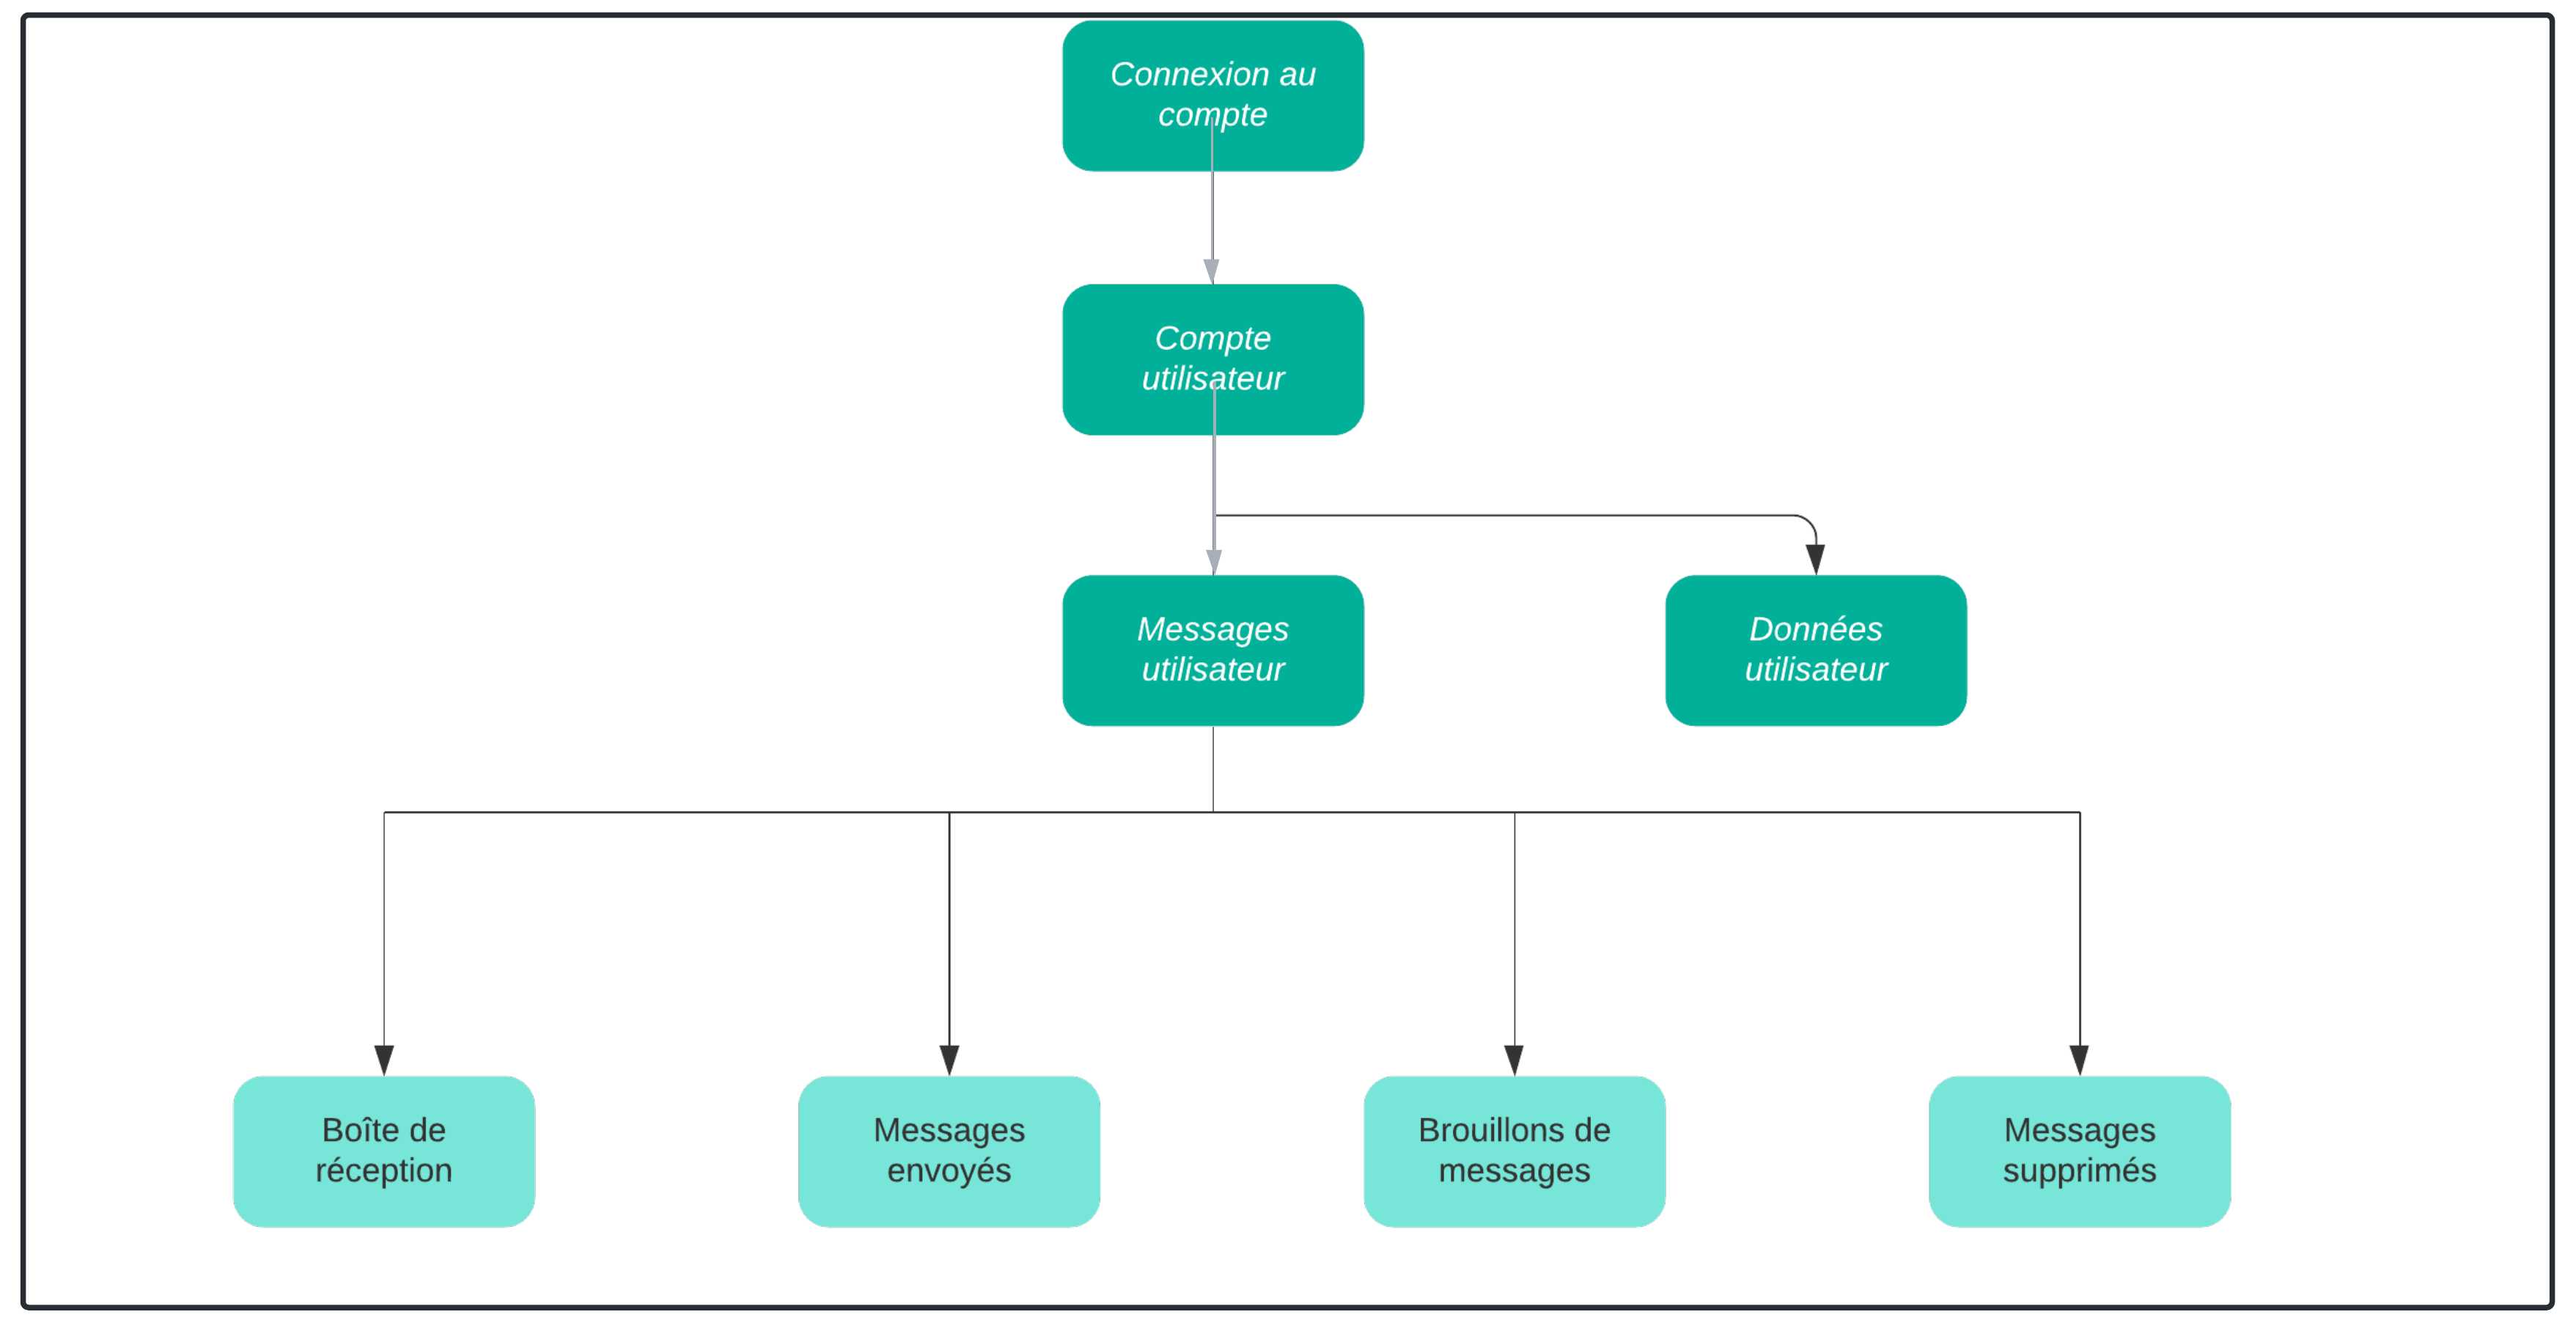
\includegraphics[width=0.88\textwidth]{Architecture de notre application}
    \caption{Architecture simplifiée de notre application}
    \label{fig:Architecture}
\end{figure}
\subsection{\LARGE Messages}
\LARGE Une collection de messages spécifiques à un utilisateur ou à plusieurs utilisateurs classés dans leur propre catégorie (reçus, envoyés, supprimés, brouillon).\\
Pour une application de messagerie, ce sont les données les plus cruciales, à cause de cela, nous avons dû choisir la meilleure construction de cette classe.\\
Dans notre application, un message ou un e-mail est une classe constitué de différents attributs notamment un identifiant message, contenu de message, destinataire, expéditeur ...\\
Voir la figure 2.2 pour la liste complète des attributs.\\
\subsection{\LARGE Base de données}
\LARGE La partie la plus importante de notre projet, l'accès en lecture ou en écriture aux données détermine la vitesse de performance de notre application, il peut donc limiter la fonctionnalité de notre application.\\
Pour cela, nous nous sommes assurés de choisir la meilleure structure pour notre base de données en mettant l'accent sur la vitesse et les performances optimales.\\
La figure ci-dessous montre une structure simplifiée de notre base de données.
Cette figure montre également la structure des parties principales de notre projet, les classes utilisateur et message ainsi que diverses autres classes nécessaires au fonctionnement de notre application.\\
Notre base de données est une base de données NoSQL, elle ne contient pas de tables.
\begin{figure}[H]
	\centering
    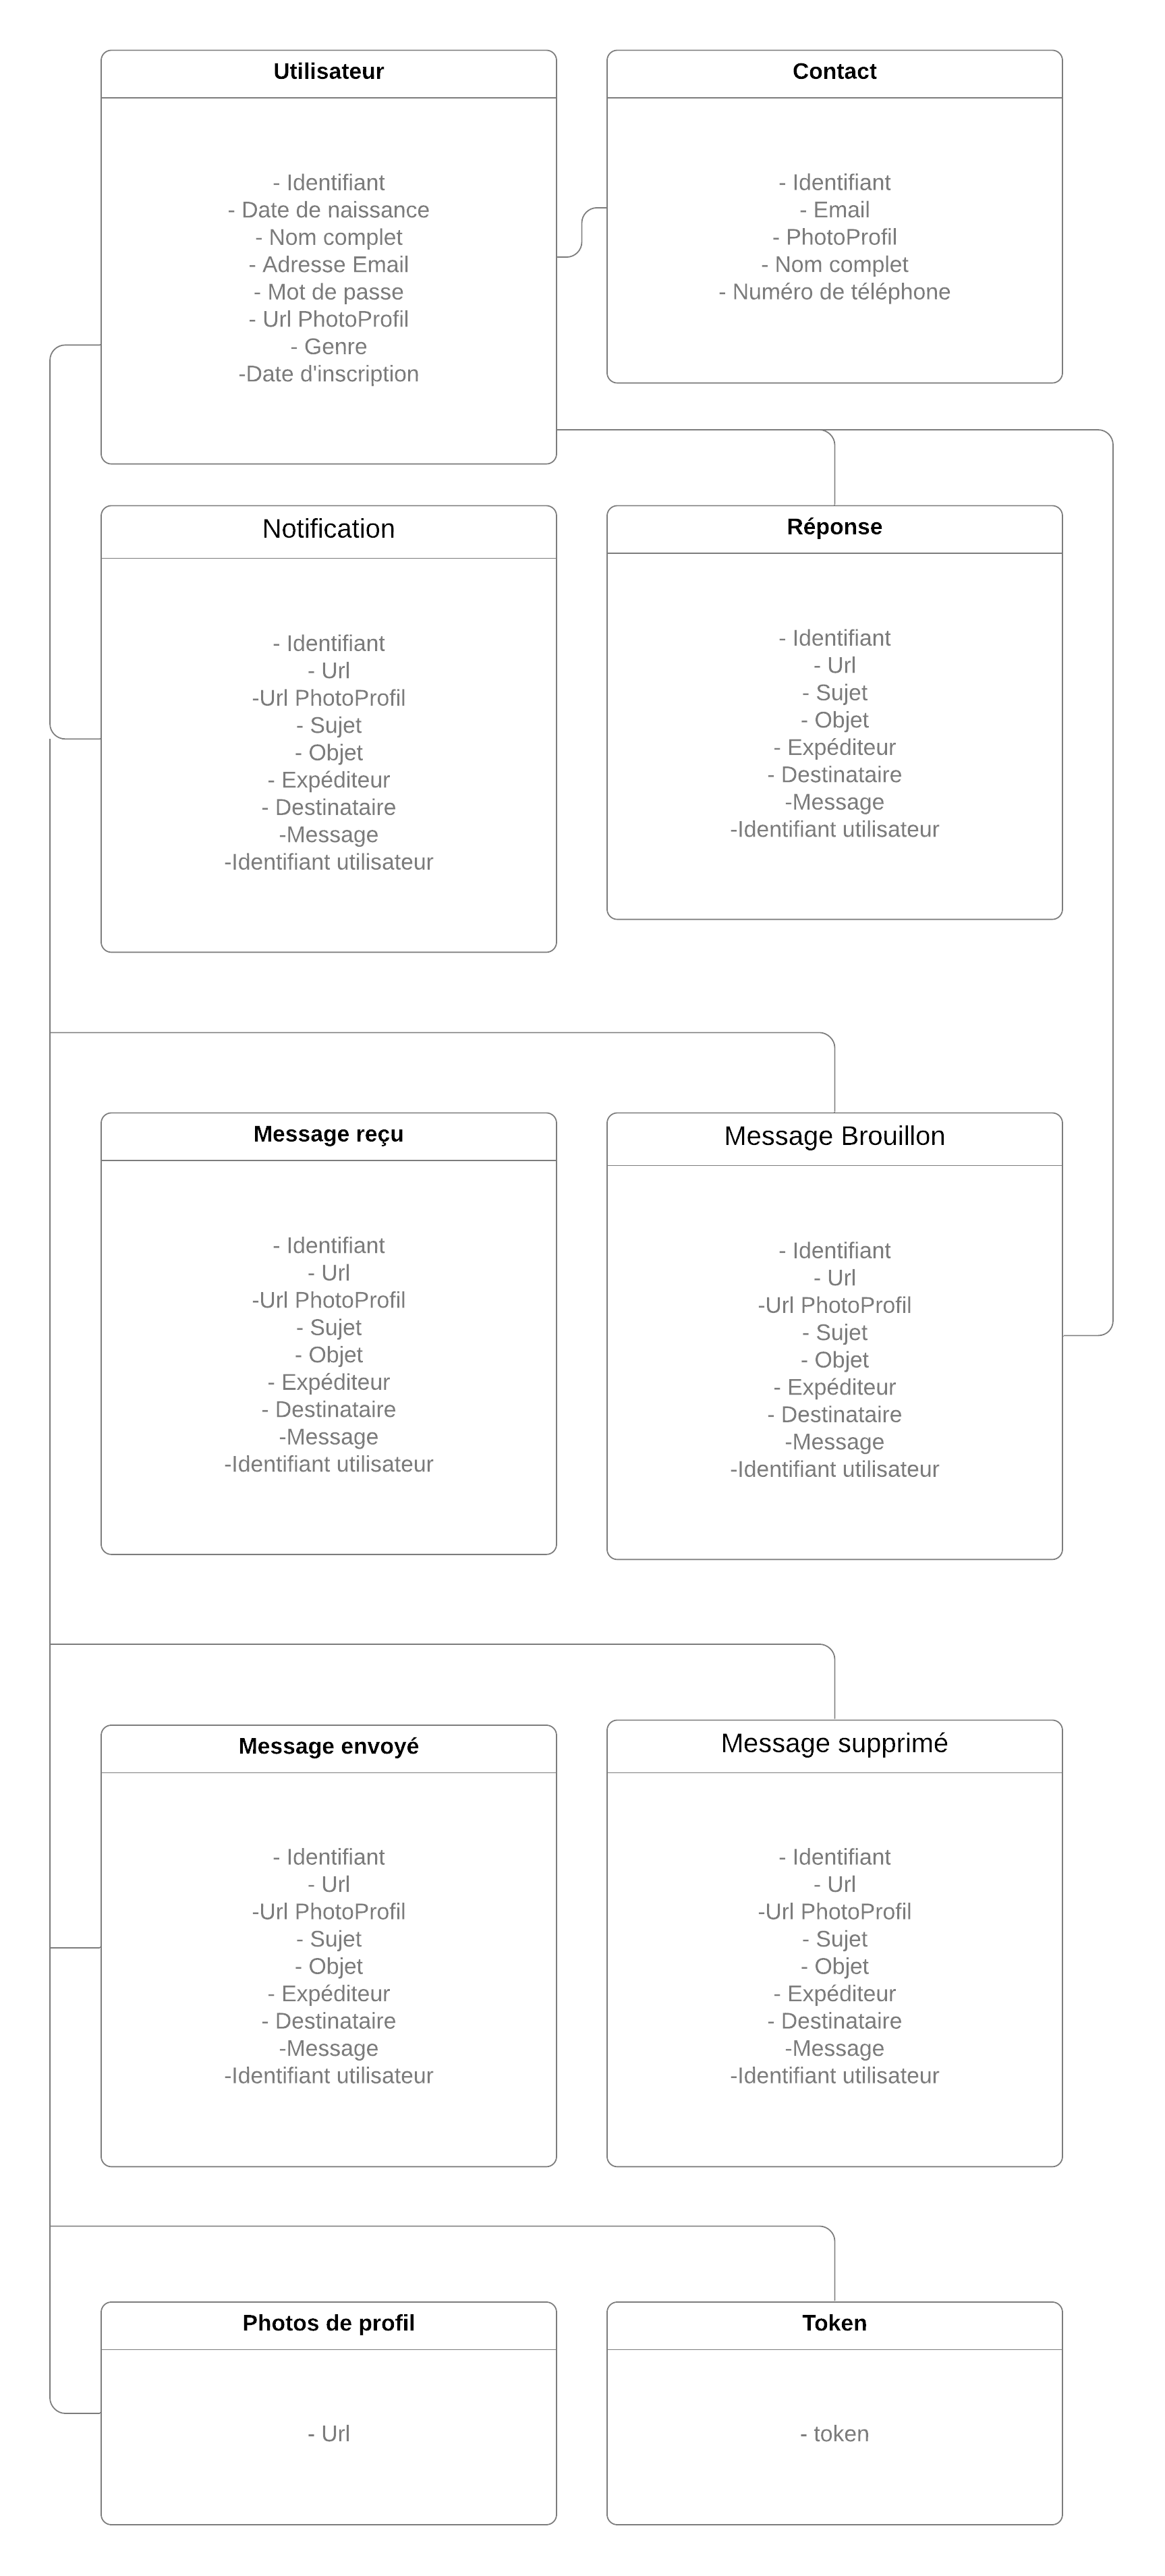
\includegraphics[scale=0.18 ]{Représentation simplifiée de notre base de données}
    \caption{Représentation simplifiée de notre base de données}
    \label{fig:Representation}
\end{figure}
\section{\huge La Modélisation de notre application :}
\subsection{\LARGE Diagramme des cas d'utilisation }
\LARGE L'objectif de ce diagramme de cas d'utilisation est de montrer globalement comment l'utilisateur pourra interagir avec notre projet une fois finalisé.\\
\begin{figure}[H]
    \centering
    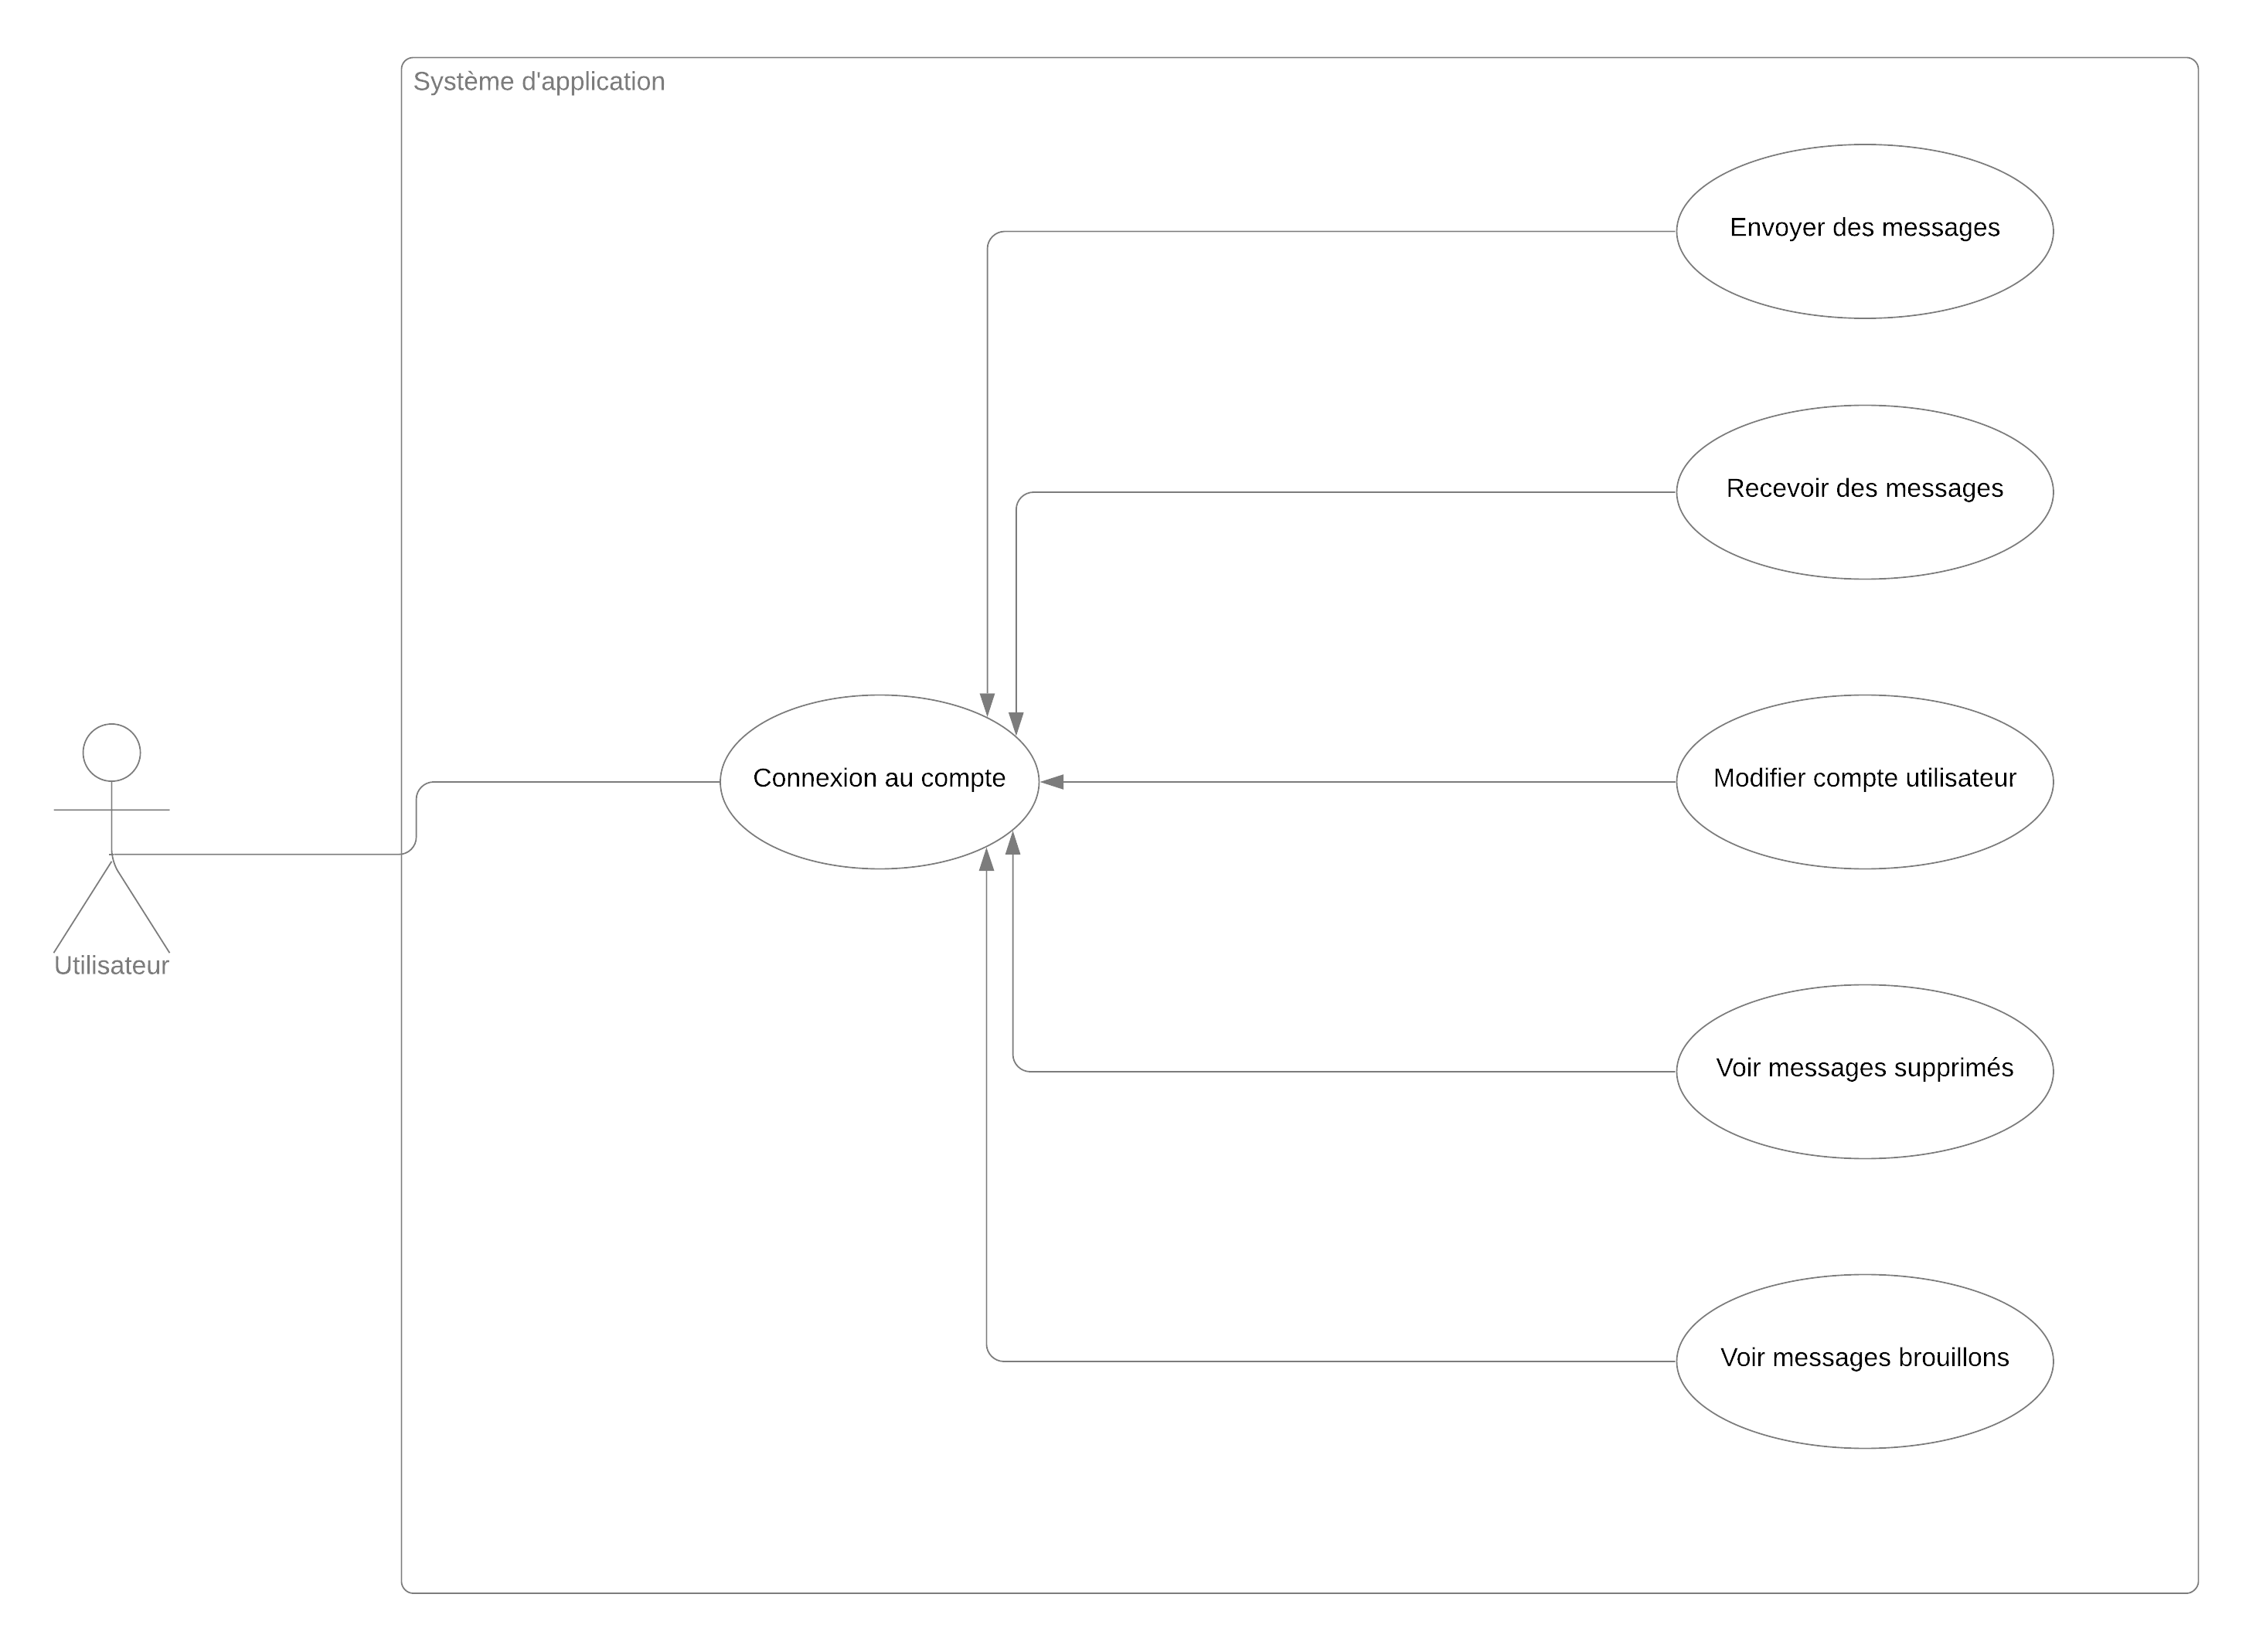
\includegraphics[width=1\textwidth]{DCU}
    \caption{Diagramme des cas d'utilisation}
    \label{fig:DCU}
\end{figure}
\subsection{\LARGE Diagramme d'activité (UML)}
\LARGE Dans UML, un diagramme d’activité est utilisé pour afficher la séquence des activités. Les diagrammes d’activité représentent le flux de travail à partir d’un point de départ au point d’arrivée. Détaillant les nombreux sentiers de décision, qui existent dans la progression des événements contenus dans l’activité. Ils peuvent être utilisés à des situations de détail, où le traitement parallèle peut survenir dans l’exécution de certaines activités.\\\\
Ce diagramme ci-dessous est le diagramme d'activité de notre activité principale (authentification), cette activité est présentée à l'utilisateur lors de la première ouverture de l'application, l'utilisateur peut alors interagir avec cette activité en se connectant ou en créant un compte.\\\\
Le déplacement entre ces activités est déterminé automatiquement par l'application en fonction des actions précédentes de l'utilisateur.
\begin{figure}[H]
    \centering
    \includegraphics[width=1\textwidth]{Diagramme d'activités}
    \caption{Diagramme d'activités principales}
    \label{fig:activity}
\end{figure}
Après l'accès au compte, l'utilisateur pourra interagir avec l'application et toutes les données en relation avec son compte en utilisant d'autres activités.
\subsection{\LARGE Conclusion}
\LARGE Cette partie nous a permis d'acquérir les connaissances nécessaires sur les différents défis auxquels nous sommes confrontés dans notre projet et a façonné notre vision de notre application et nous a aidés à identifier ses besoins.\\
Dans le chapitre suivant, nous passerons à l'implémentation de notre application en utilisant le langage de programmation choisi (JAVA) et l'IDE Android Studio.

\end{document}